\documentclass[a4paper, 11pt]{article}
\usepackage[utf8]{inputenc}
\usepackage[T1]{fontenc}
\usepackage[english]{babel}
\usepackage{graphicx}

\usepackage{hyperref}

\pagestyle{headings}
\setlength{\hoffset}{-50pt}  
\setlength{\textwidth}{470pt}
\setlength{\textheight}{700pt}
\setlength{\topmargin}{0pt}

\title{KAMISADO}
\author{Valentin BENOZILLO, Mathieu VIOLA, Rémi VIOLA}
\date{\today}

\begin{document}

\maketitle

\begin{abstract}
This report will present you the game Kamisado as well as various artificial intelligences and heuristics which we programmed.
\end{abstract}

\newpage

\tableofcontents

\newpage

\section{Presentation of the game}
\verb?Kamisado? \footnote{\url{http://www.burleygames.com/board-games/kamisado-original/}} is an abstract two-player game where, to win a round, you have to move, on a 8$\times$8 colored board, one of your 8 colored towers from an edge to the other one. The rules are simple.\\
In your turn, you can move your tower of the active color, in a straight line, of the number of square which you want. The active color is the color of the square where your opponent arrived during the previous move.\\
The party can be played in one, three, seven or fifteen rounds. To simplify the project, we decided to code only one round.
\begin{center}
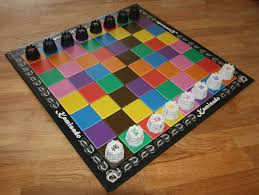
\includegraphics[scale = 0.09]{kamisado.jpeg}
\end{center}

\section{Graphical User Interface}
To make our project more alive, we created a graphical user interface with the library \verb?xpce? \footnote{\url{http://www.swi-prolog.org/packages/xpce/}} of SWI-Prolog.\\
\begin{center}
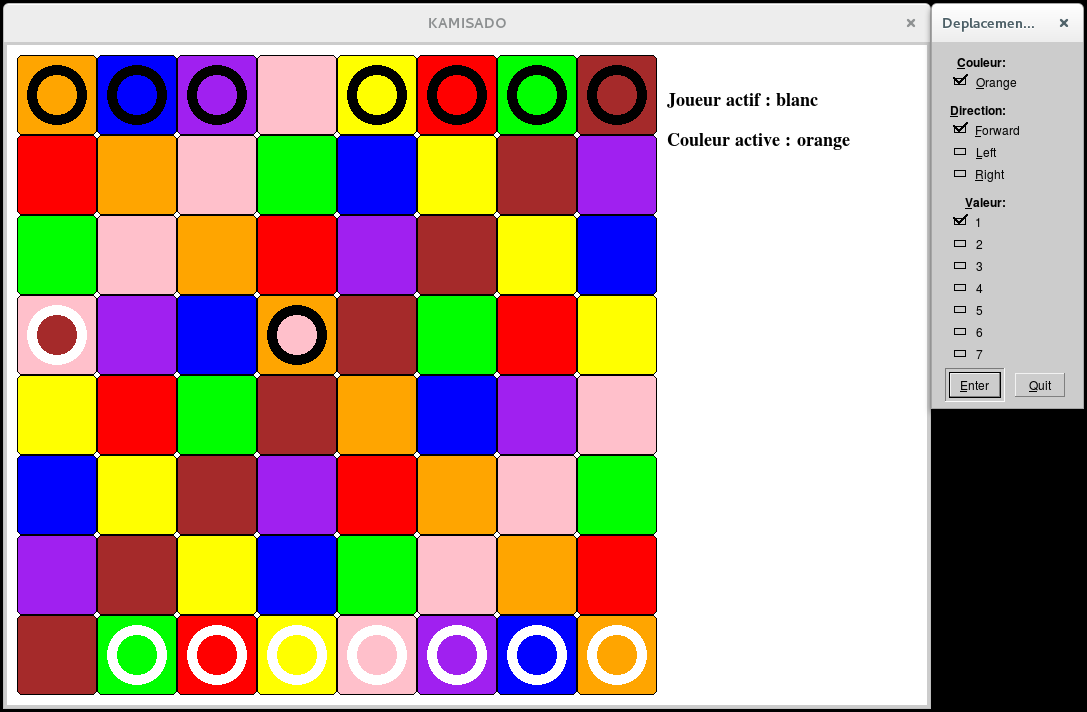
\includegraphics[scale = 0.30]{kamisado.png}
\end{center}
To run our program in a terminal, you have to write :
\begin{center}
\verb?swipl k.pl?
\end{center}
In Prolog, you have to call the predicate \verb?commencer(firstname).? if you want to start or the predicate \verb?ia_commencer(firstname).? if you want to let the artificial intelligence start where firstname is one of our first name. 
During the game, to play, you have to click on one of your towers and checkboxes will pop up. You have to select the color of the tower (only for the first round if you start), the direction  between left, forward and right, and the number of square of your move.
You have a printing of the current player and the current color and, if it's the end of the round, a printing for the winning or the loss of the round.\\
You can replay with the predicates \verb?recommencer(firstname).? and \verb?ia_recommencer(firstname).?
This interface is basic but sufficient for seeing what you do.

\section{Heuristics}
\subsection{remi}
This heuristic is the simplest. The artificial intelligence selects all the squares where it can move without risks to lose. In this list, it selects the first square which allows to win at the following move by the active tower.\\
If there is no possible square with this constraint, it selects the first square which forces the player to free a square which allows to win at the following move by the active tower.\\
If there is no square which satisfy this new constraint, it selects the first square in the list.\\
In the case there would be no playable square without risks, it knows that it will lose and it also chooses the first one of the list.\\ \\
To test this strategy, you have several possibilities. If the artificial intelligence starts, it chooses the first color randomly but you can see that, for each color, it move on the nearest square where it can force the user to move.
If you start, you can try this fatal first move : 
\begin{verbatim}
brown-forward-6 !
\end{verbatim}
The artificial intelligence move to the brown square of the second line but you can't play your brown tower. So, you pass and it have to play its red tower which wins.\\
For more interesting tests when you start, you can try :
\begin{verbatim}
red-forward-4 + blue-forward-3 + orange-left-5 + pink-forward-5 + red-left-1...
\end{verbatim}
After the first move, the artificial intelligence forces you to move your blue tower because it can't have an attack position. After the second, it move to a position where it will attack directly with its active tower when you will let it play this tower.
After the third, it moves its orange tower to the pink square because it's the nearest postition where it can force you to free a square to attack. It doesn't choose the blue square because it would let you win. After each other move, the artificial intelligence move to have an attack position. 
In this situation, you just have the yellow square free for your brown tower... But you can win with the following sequence : 
\begin{verbatim}
...brown-forward-3 + yellow-right-2 + pink-forward-2
\end{verbatim}
The first move is compulsory. The second asks to the artificial intelligence to move its orange tower which is blocked. The third go to the goal.

\subsection{valentin}


\subsection{mathieu}


\subsection{mathieu2}
Contrary to the previous version, we do not count any more the accessible final squares but the number of towers which can win at their next move. 
With this heuristics, the first moves are the same but as soon as possible, the artificial intelligence tries finally to increase the number of empty squares on the last line.

\subsection{mathieu3}
In this version, we decided to take into account also the number of accessible final squares of the opponent as a penalty in our evaluation.

\subsection{mathieu4}
In this final version, we decided to increase the evaluation by 20 times the difference between the number of accessible squares for the player and for the artificial intelligence. We also increase this evaluation by the difference between the number of accessible final squares by each of them.

\end{document}
